\section{Experimental Results}
\label{sec:experiments}

We evaluate Kimodo-Policy's control performance and deployment feasibility through single- and multi-task experiments on HumanoidArena (Sec.~\ref{sec:exp_simulation}), manipulation tasks on SIMPLE (Sec.~\ref{sec:exp_simple}), and real-world deployment (Sec.~\ref{sec:exp_real}). We then examine T2M backbone quality (Sec.~\ref{sec:exp_t2m}), data and model scaling (Sec.~\ref{sec:exp_scaling}), and key design choices through ablations (Sec.~\ref{sec:exp_ablation}). Details of the datasets, training protocols, and evaluation environments are provided in Appendix~\ref{sec:experimental_setup}.

\subsection{Evaluation on the HumanoidArena Benchmark}
\label{sec:exp_simulation}

HumanoidArena~\cite{humanoidarena} comprises seven language-conditioned humanoid tasks spanning human--object interaction (HOI) and human--scene interaction (HSI). Task visualizations are provided in Appendix~\ref{sec:vis_humanoidarena} (Fig.~\ref{fig:humanoidarena}). We evaluate Kimodo-Policy in two settings: independent fine-tuning on each task and joint training across multiple SONIC tasks, covering single-task capability and the more challenging multi-task setting.



\begingroup
\setlength{\intextsep}{6pt plus 1pt minus 1pt}
\textbf{Single-task results.} We fine-tune one policy per task with RTC disabled to match baselines. Kimodo-Policy uses direct task fine-tuning; Kimodo-Policy$^{*}$ initializes ControlNet and the hand head from our 419-hour VLA pretraining. Kimodo-Policy achieves the highest overall success rate (SR; 69.51\%), exceeding the strongest baseline, DP~\cite{chi2023diffusionpolicy} (60.0\%), by 9.51 percentage points. It also leads in average HSI SR (84.58\%) and ties Kimodo-Policy$^{*}$ for lowest average fall rate (AFR; 4.29\%). Kimodo-Policy$^{*}$ achieves 67.14\% overall and 84.17\% average HSI SR, leading OpenDoor (93.3\%) and VisNavi (76.7\%). VLA pretraining improves selected tasks, while direct fine-tuning yields higher overall SR.




  




\begin{table}[H]
  \setlength{\belowcaptionskip}{6pt}
  \caption{\textbf{\textit{Single-task HumanoidArena results.}} A separate policy is fine-tuned per task. For Tables~\ref{tab:arena_single_task}--\ref{tab:arena_multi_task}, values are mean $\pm$ standard deviation; $^{*}$ marks VLA-pretrained initialization, and bold/underlined entries mark best/second-best results.}
  \label{tab:arena_single_task}
  \centering
  \arrayrulecolor{hclblue}
  \begin{adjustbox}{max width=\textwidth}
  \setlength{\tabcolsep}{4.2pt}
  \renewcommand{\arraystretch}{1.08}

  \begin{tabular}{ccccc|ccccc}
  \toprule
  & &
  \multicolumn{3}{c|}{\textbf{Human--Object Interaction}} &
  \multicolumn{4}{c}{\textbf{Human--Scene Interaction}} & \\
  \cmidrule(lr){3-5}
  \cmidrule(lr){6-9}

  \multirow{-2}{*}{\textbf{Method}} &
  \multirow{-2}{*}{\textbf{AFR~($\downarrow$)}} &
  \textbf{\textsc{Football}} &
  \textbf{\textsc{DoubleDesk}} &
  \textbf{\textsc{P\&Pbox}} &
  \textbf{\textsc{OpenDoor}} &
  \textbf{\textsc{SitSofa}} &
  \textbf{\textsc{Boxing}} &
  \textbf{\textsc{VisNavi}} &
  \multirow{-2}{*}{\textbf{\textsc{Overall~($\uparrow$)}}} \\
  
  \midrule
  ACT~\cite{ACT}
  & 8.57\%
  & 16.7$\pm$6.2\%
  & 18.3$\pm$4.7\%
  & 56.7$\pm$6.2\%
  & 78.3$\pm$9.4\%
  & 73.3$\pm$8.5\%
  & 56.7$\pm$6.2\%
  & 33.3$\pm$2.4\%
  & 47.61\% \\

  DP~\cite{chi2023diffusionpolicy}
  & 8.33\%
  & \textbf{45.0$\pm$10.8\%}
  & 36.7$\pm$4.7\%
  & 75.0$\pm$4.1\%
  & 85.0$\pm$10.8\%
  & 78.3$\pm$14.3\%
  & \textbf{76.7$\pm$2.4\%}
  & 23.3$\pm$6.2\%
  & 60\% \\

  FM~\cite{FM_objective}
  & 5.71\%
  & 13.3$\pm$2.4\%
  & 38.3$\pm$4.7\%
  & 73.3$\pm$6.2\%
  & 70.0$\pm$4.1\%
  & 15.0$\pm$14.7\%
  & 70.0$\pm$8.2\%
  & 38.3$\pm$14.3\%
  & 45.46\% \\

  $\pi_{0.5}$~\cite{pi05}
  & \underline{5.24\%}
  & 10.0$\pm$4.1\%
  & \textbf{43.3$\pm$6.2\%}
  & 71.7$\pm$11.8\%
  & 66.7$\pm$6.2\%
  & 73.3$\pm$2.4\%
  & 70.0$\pm$0.0\%
  & 23.3$\pm$6.2\%
  & 51.19\% \\

  \rowcolor{hclbrown!8!white}
  \texttt{Ours}
  & \textbf{4.29\%}
  & \underline{28.3$\pm$6.2\%}
  & \underline{40.0$\pm$0.0\%}
  & \textbf{80.0$\pm$4.1\%}
  & \underline{90.0$\pm$4.1\%}
  & \textbf{100.0$\pm$0.0\%}
  & \underline{73.3$\pm$13.1\%}
  & \underline{75.0$\pm$10.8\%}
  & \textbf{69.51\%} \\


  \rowcolor{hclbrown!15!white}
  \texttt{Ours}$^{*}$
  & \textbf{4.29\%}
  & 26.7$\pm$4.7\%
  & 28.3$\pm$2.4\%
  & \underline{78.3$\pm$8.5\%}
  & \textbf{93.3$\pm$2.4\%}
  & \underline{96.7$\pm$2.4\%}
  & 70.0$\pm$8.2\%
  & \textbf{76.7$\pm$18.9\%}
  & \underline{67.14\%} \\

  \bottomrule
  \end{tabular}
  \end{adjustbox}
\end{table}


\textbf{Multi-task results.} We jointly train one policy on all seven HumanoidArena tasks and evaluate under SONIC~\cite{humanoidarena,sonic}, with RTC disabled to match baselines. Table~\ref{tab:arena_multi_task} shows Kimodo-Policy$^{*}$ reaching 72.14\% overall SR, exceeding the strongest baseline, $\pi_{0.5}$~\cite{pi05} (53.8\%), by 18.33 percentage points, with lowest AFR (4.29\%). It leads HOI (56.11\%) and HSI (84.17\%) averages, P\&Pbox (90.0\%), OpenDoor (95.0\%), SitSofa (96.7\%, tied), and VisNavi (76.7\%). Without VLA pretraining, Kimodo-Policy reaches 67.63\% overall and 51.67\% HOI SR; overall SR falls only 1.88 percentage points from single-task training. Thus, a shared policy can retain much of its single-task performance with high success and low fall rates.

\begin{table}[H]
  \setlength{\belowcaptionskip}{6pt}
  \caption{\textbf{\textit{Multi-task HumanoidArena results.}} One policy is jointly trained on all seven tasks.}
  \label{tab:arena_multi_task}
  \centering
  \arrayrulecolor{hclblue}
  \begin{adjustbox}{max width=\textwidth}
  \setlength{\tabcolsep}{4.2pt}
  \renewcommand{\arraystretch}{1.08}

  \begin{tabular}{ccccc|ccccc}
  \toprule
  & &
  \multicolumn{3}{c|}{\textbf{Human--Object Interaction}} &
  \multicolumn{4}{c}{\textbf{Human--Scene Interaction}} & \\
  \cmidrule(lr){3-5}
  \cmidrule(lr){6-9}

  \multirow{-2}{*}{\textbf{Method}} &
  \multirow{-2}{*}{\textbf{AFR~($\downarrow$)}} &
  \textbf{\textsc{Football}} &
  \textbf{\textsc{DoubleDesk}} &
  \textbf{\textsc{P\&Pbox}} &
  \textbf{\textsc{OpenDoor}} &
  \textbf{\textsc{SitSofa}} &
  \textbf{\textsc{Boxing}} &
  \textbf{\textsc{VisNavi}} &
  \multirow{-2}{*}{\textbf{\textsc{Overall~($\uparrow$)}}} \\
  \midrule

  ACT~\cite{ACT}
  & 7.4\%
  & 20.0$\pm$4.1\%
  & 30.0$\pm$4.1\%
  & 60.0$\pm$12.2\%
  & 58.3$\pm$2.4\%
  & 21.7$\pm$2.4\%
  & 58.3$\pm$10.3\%
  & 28.3$\pm$4.7\%
  & 39.5\% \\

  DP~\cite{chi2023diffusionpolicy}
  & 7.1\%
  & \textbf{53.3$\pm$6.2\%}
  & 35.0$\pm$10.8\%
  & 0.0$\pm$0.0\%
  & 83.3$\pm$6.2\%
  & \underline{83.3$\pm$4.7\%}
  & 21.7$\pm$30.6\%
  & 50.0$\pm$14.7\%
  & 46.7\% \\

  FM~\cite{FM_objective}
  & 7.1\%
  & 21.7$\pm$8.5\%
  & 20.0$\pm$7.1\%
  & 0.0$\pm$0.0\%
  & 76.7$\pm$2.4\%
  & 48.3$\pm$6.2\%
  & 18.3$\pm$25.9\%
  & 38.3$\pm$6.2\%
  & 31.9\% \\

  $\pi_{0.5}$~\cite{pi05}
  & 6.4\%
  & 10.0$\pm$7.1\%
  & 30.0$\pm$7.1\%
  & 75.0$\pm$4.1\%
  & 85.0$\pm$4.1\%
  & 70.0$\pm$14.7\%
  & \textbf{71.7$\pm$12.5\%}
  & 35.0$\pm$4.1\%
  & 53.8\% \\

  \rowcolor{hclbrown!8!white}
  \texttt{Ours}
  & \underline{5.0\%}
  & 35.0$\pm$7.1\%
  & \textbf{40.0$\pm$0.0\%}
  & \underline{80.0$\pm$4.1\%}
  & \underline{93.3$\pm$6.2\%}
  & \textbf{96.7$\pm$4.7\%}
  & 66.7$\pm$4.7\%
  & \underline{61.7$\pm$6.2\%}
  & \underline{67.6\%} \\


  \rowcolor{hclbrown!15!white}
  \texttt{Ours}$^{*}$
  & \textbf{4.3\%}
  & \underline{40.0$\pm$4.1\%}
  & \underline{38.3$\pm$2.4\%}
  & \textbf{90.0$\pm$4.1\%}
  & \textbf{95.0$\pm$4.1\%}
  & \textbf{96.7$\pm$4.7\%}
  & \underline{68.3$\pm$10.3\%}
  & \textbf{76.7$\pm$8.5\%}
  & \textbf{72.1\%} \\



  \bottomrule
  \end{tabular}
  \end{adjustbox}
\end{table}


\textbf{Attention map analysis.} Figure~\ref{fig:attention} shows Kimodo-Policy focusing on the ball in Football, box in P\&P Box, and punching bag in Boxing, alongside relevant scene elements for door opening, sitting, and navigation. $\pi_{0.5}$ responds less locally, while Diffusion Policy activates broader scene regions. This task-dependent focus suggests alignment with instruction semantics and use of task-relevant cues for shared multi-task action selection.

\begin{figure}[H]
  \centering
  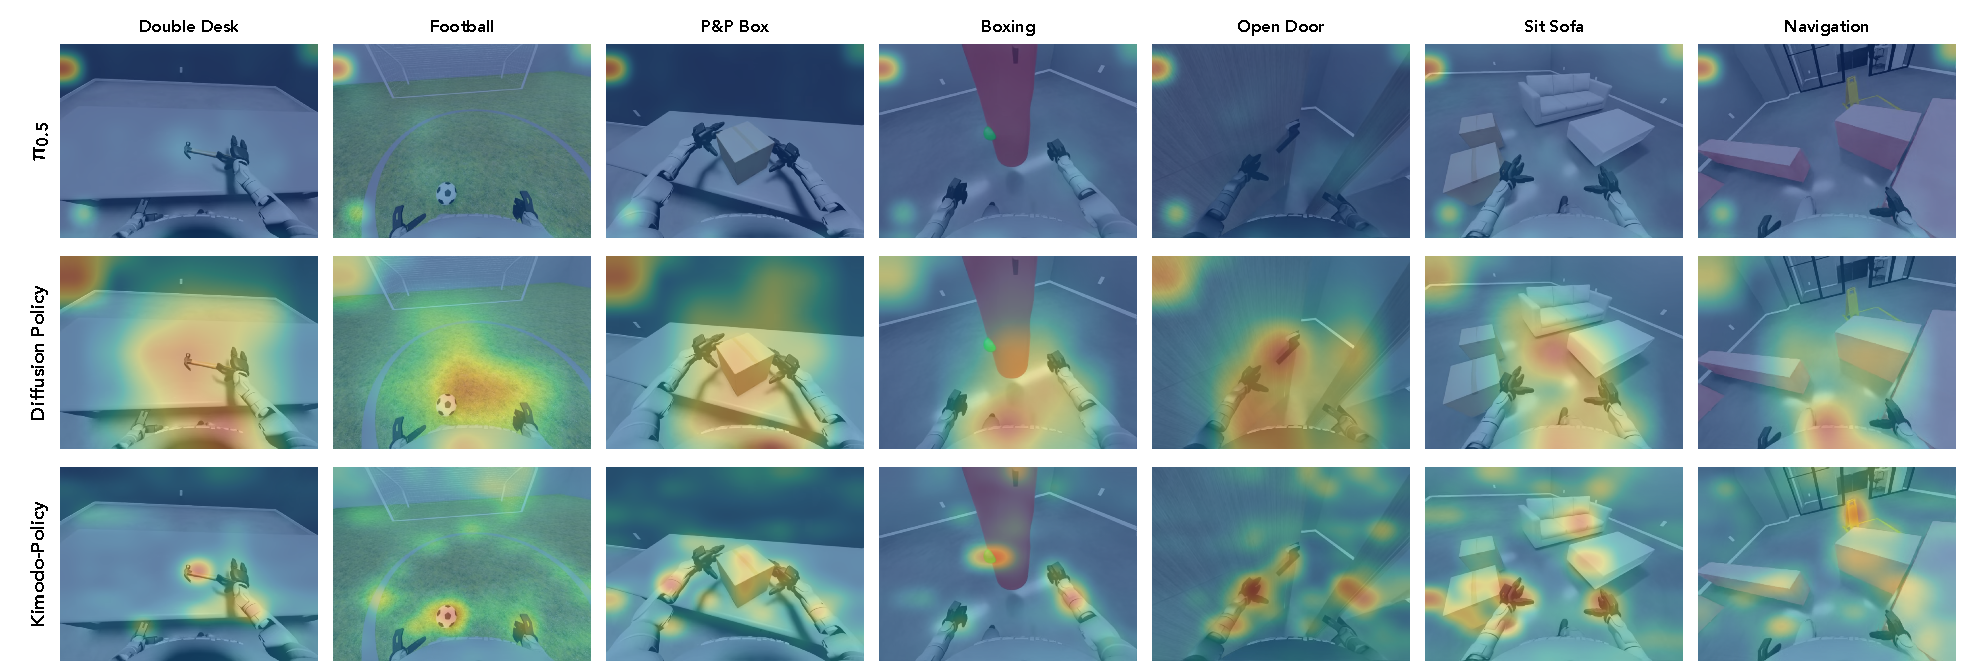
\includegraphics[width=\textwidth]{image/attention.pdf}
  \caption{\textbf{Task-Conditioned Visual Attention.} Columns show seven HumanoidArena tasks; rows (top to bottom) show $\pi_{0.5}$, Diffusion Policy, and Kimodo-Policy. Kimodo-Policy shifts attention toward task-relevant objects and interaction regions.}
  \label{fig:attention}
\end{figure}
\endgroup

\subsection{Evaluation on the Simple Benchmark}
\label{sec:exp_simple}
We further evaluate Kimodo-Policy on the SIMPLE benchmark~\cite{simple}, using the L0--L2 protocol with progressively stronger visual, lighting, and target-pose randomization~\cite{simple}. We fine-tune an independent policy for each of the eight benchmark tasks and report the results in Table~\ref{table:simple_main_results}. This protocol isolates skill acquisition while testing robustness under increasing distribution shifts. See Appendix~\ref{sec:vis_simple} (Fig.~\ref{fig:simple_tasks}) for task visualizations.



\textbf{Single-task results.} Table~\ref{table:simple_main_results} evaluates VLA-pretrained Kimodo-Policy (\texttt{Ours}$^{*}$) on eight SIMPLE tasks, aggregating L0--L2 success rates with RTC disabled to match the baselines. It achieves best or joint-best results on six tasks: Handover (83\% vs. 80\% for the strongest baseline), Mobile P\&P (70\% vs. 60\%), OpenOven (57\% vs. 53\%), OpenFaucet (53\% vs. 33\%), CloseDoor and Push Office Chair (both 100\%, tied with $\Psi_0$). It ranks second on XMoveBendPick (80\% vs. 93\% for $\Psi_0$) and OpenTrashCan (63\% vs. 83\%). These results show that the motion-prior-based, visually grounded root--body--hand policy supports handover, mobile manipulation, articulated-object interaction, and pushing under visual, lighting, and target-pose variation.

\begin{table}[H]
  \setlength{\belowcaptionskip}{6pt}
  \caption{\textbf{\textit{Single-Task Results on SIMPLE.}} L0--L2 progressively increase visual and lighting variation and target-pose randomization. Entries report L0/L1/L2 success counts and aggregate success rates (parentheses); bold/underlined values mark the best/second-best aggregate rates.}
  \label{table:simple_main_results}
  \centering
  \arrayrulecolor{hclblue}
  \setlength{\tabcolsep}{0pt}
  \renewcommand{\arraystretch}{1.08}
  \fontsize{6.2}{7}\selectfont
  \newcommand{\taskheader}[1]{{\fontsize{5.55}{6.2}\selectfont\textbf{\textsc{\hspace{2.2pt}#1\hspace{2.2pt}}}}}
  \newcommand{\resultentry}[2]{{\fontsize{5.2}{6}\selectfont\hspace{2.2pt}#1\;(#2)\hspace{2.2pt}}}
  \newcommand{\bestentry}[2]{{\fontsize{5.2}{6}\selectfont\textbf{\hspace{2.2pt}#1\;(#2)\hspace{2.2pt}}}}
  \newcommand{\secondentry}[2]{{\fontsize{5.2}{6}\selectfont\hspace{2.2pt}\underline{#1\;(#2)}\hspace{2.2pt}}}

  \begin{adjustbox}{width=\textwidth}
  \begin{tabular}{@{}c*{8}{c}@{}}
    \toprule
    {\fontsize{5.55}{6.2}\selectfont\textbf{Method}}
    & \taskheader{Handover}
    & \taskheader{Mobile P\&P}
    & \taskheader{XMoveBendPick}
    & \taskheader{CloseDoor}
    & \taskheader{OpenOven}
    & \taskheader{OpenFaucet}
    & \taskheader{Push Office Chair}
    & \taskheader{OpenTrashCan} \\
    \midrule

    $\Psi_0$~\cite{psi0}
    & \secondentry{7/7/10}{80\%}
    & \secondentry{7/5/6}{60\%}
    & \bestentry{10/9/9}{93\%}
    & \bestentry{10/10/10}{100\%}
    & \secondentry{7/5/4}{53\%}
    & \secondentry{3/3/4}{33\%}
    & \bestentry{10/10/10}{100\%}
    & \bestentry{7/9/9}{83\%} \\

    \rowcolor{hclbrown!15!white}
    \texttt{Ours}$^{*}$
    & \bestentry{9/8/8}{83\%}
    & \bestentry{9/8/4}{70.0\%}
    & \secondentry{10/7/7}{80\%}
    & \bestentry{10/10/10}{100\%}
    & \bestentry{8/4/5}{57\%}
    & \bestentry{5/6/5}{53\%}
    & \bestentry{10/10/10}{100\%}
    & \secondentry{9/4/6}{63\%} \\

    \bottomrule
  \end{tabular}
  \end{adjustbox}
\end{table}


\subsection{Evaluation on the Real-World Humanoid Robot}
\label{sec:exp_real}
We deploy Kimodo-Policy on a physical humanoid robot to assess language-conditioned loco-manipulation under unconstrained sensing and execution conditions. The evaluation covers eight tasks that require different combinations of locomotion, balance maintenance, single- and dual-arm coordination, and contact-rich manipulation. See Appendix~\ref{sec:vis_real_world} (Fig.~\ref{fig:real_world}) for representative real-world tasks illustrating coordinated whole-body motion and manipulation during physical-robot execution. For each task, we execute ten trials and record the number of successful completions, providing a direct measure of deployment reliability across heterogeneous real-world interactions.



\textbf{Real-world results.} Figure~\ref{fig:real_world_success_rates} compares task-level success across the eight physical-robot tasks. Kimodo-Policy trained from scratch achieves a mean success rate of 45\%, exceeding the reported averages of GR00T N1.6~\cite{grootn1} (31\%) and $\Psi_0$~\cite{psi0} (35\%). Initializing Kimodo-Policy with VLA-pretrained weights further raises the mean success rate to 60\%, a 15-percentage-point gain over the scratch-trained model. This gain is reflected across tasks: the pretrained policy improves success on seven tasks and matches the scratch model on Cart Pushing (60\%). Its strongest results are on Punching Bag (90\%), Cushion Sitting (80\%), and Dual-Arm PNP (70\%). Overall, the results indicate that VLA pretraining provides a useful initialization for adapting Kimodo-Policy to diverse real-world humanoid tasks, improving average performance while retaining competitive task-level success.

\begin{figure}[H]
  \centering
  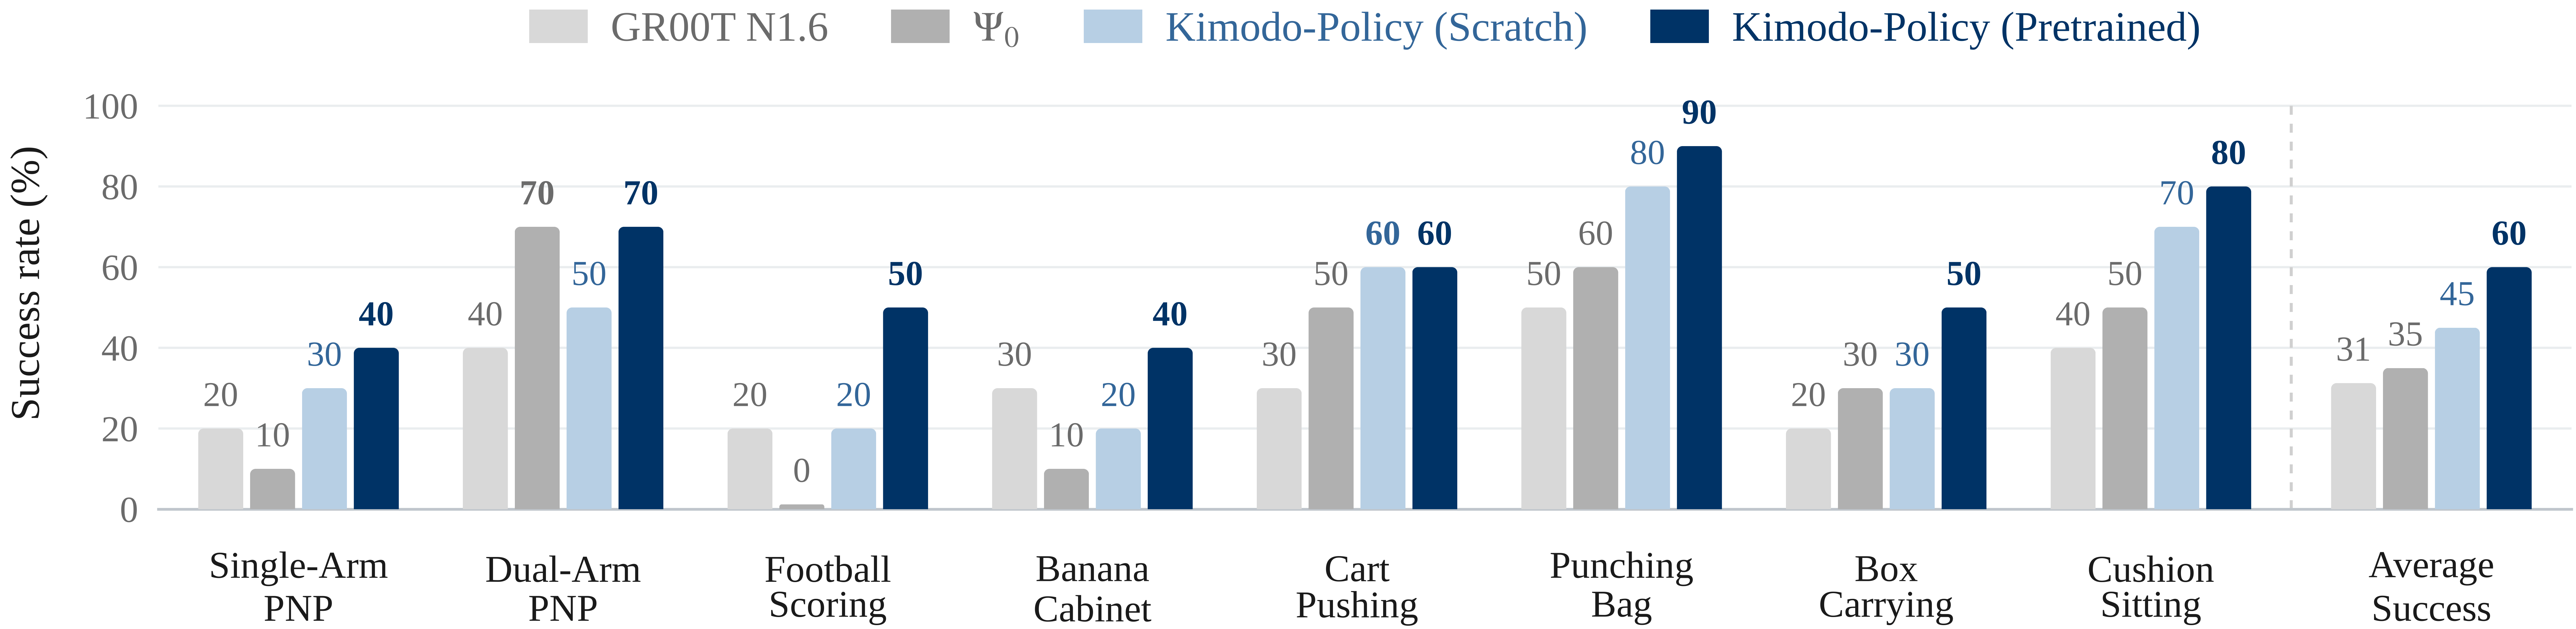
\includegraphics[width=\textwidth]{image/real_world_success_rates.png}
  \caption{\textbf{Real-World Success Rates Across Eight Tasks.} The plot compares GR00T N1.6, $\Psi_0$, and Kimodo-Policy trained from scratch or initialized with VLA pretraining. Bars report the success rate for each task; the rightmost group gives the mean across all eight tasks.}
  \label{fig:real_world_success_rates}
\end{figure}

\subsection{Does Better T2M Improve VLA Performance?}
\label{sec:exp_t2m}
Kimodo-Policy uses the pretrained Kimodo T2M model~\cite{kimodo} as its motion backbone. To assess how prior quality affects VLA control, we compare Kimodo-G1-SEED-v1 and RP-v1 under the same policy architecture, adaptation procedure, and HumanoidArena protocol. Both have 282M parameters and 90\%/10\% train/test splits; SEED-v1 uses 288\,h of BONES-SEED motion data, whereas RP-v1 uses 700\,h of Rigplay~\cite{kimodo}.
\begin{table}[H]
  \setlength{\belowcaptionskip}{6pt}
  \caption{
    \textbf{\textit{Effect of the T2M backbone on Kimodo-Policy.}} We compare two same-size Kimodo-G1 backbones using the same adaptation protocol. Data scales include the training and test splits; results are mean $\pm$ standard deviation over three seeds.}
  \label{tab:t2m_dependency}
  \centering
  \arrayrulecolor{hclblue}
  \begin{adjustbox}{max width=\textwidth}
  \setlength{\tabcolsep}{3.8pt}
  \renewcommand{\arraystretch}{1.08}

  \begin{tabular}{cccccc|ccccc}
  \toprule
  \multirow{2}{*}{\textbf{Base Model}} &
  \multirow{2}{*}{\textbf{Model Size}} &
  \multirow{2}{*}{\textbf{Data Scale}} &
  \multicolumn{3}{c|}{\textbf{Human--Object Interaction}} &
  \multicolumn{4}{c}{\textbf{Human--Scene Interaction}} &
  \multirow{2}{*}{\textbf{Overall~($\uparrow$)}} \\
  \cmidrule(lr){4-6}
  \cmidrule(lr){7-10}

  & & &
  \textbf{\textsc{Football}} &
  \textbf{\textsc{DoubleDesk}} &
  \textbf{\textsc{P\&Pbox}} &
  \textbf{\textsc{OpenDoor}} &
  \textbf{\textsc{SitSofa}} &
  \textbf{\textsc{Boxing}} &
  \textbf{\textsc{VisNavi}} \\
  \midrule

  \texttt{Kimodo-G1-SEED-v1}
  & 282\,M
  & 288\,h
  & \textbf{50.00$\pm$16.33\%}
  & \underline{33.33$\pm$15.46\%}
  & \underline{75.00$\pm$10.80\%}
  & \underline{60.00$\pm$4.08\%}
  & \underline{90.00$\pm$4.08\%}
  & \textbf{71.67$\pm$8.50\%}
  & \textbf{70.00$\pm$18.71\%}
  & \underline{64.29\%} \\

  \rowcolor{hclbrown!8!white}
  \texttt{Kimodo-G1-RP-v1}
  & 282\,M
  & 700\,h
  & \underline{35.0$\pm$7.1\%}
  & \textbf{40.0$\pm$0.0\%}
  & \textbf{80.0$\pm$4.1\%}
  & \textbf{93.3$\pm$6.2\%}
  & \textbf{96.7$\pm$4.7\%}
  & \underline{66.7$\pm$4.7\%}
  & \underline{61.7$\pm$6.2\%}
  & \textbf{67.63\%} \\

  \bottomrule
  \end{tabular}
  \end{adjustbox}
\end{table}

\textbf{T2M transfer results.} Table~\ref{tab:t2m_dependency} shows task-dependent gains from the stronger backbone. Overall success rate (SR) rises from 64.29\% with Kimodo-G1-SEED-v1 to 67.63\% with RP-v1, a 3.34-point improvement. RP-v1 improves DoubleDesk from 33.33\% to 40.0\%, P\&Pbox from 75.0\% to 80.0\%, OpenDoor from 60.0\% to 93.3\%, and SitSofa from 90.0\% to 96.7\%. However, Football declines from 50.0\% to 35.0\%, Boxing from 71.67\% to 66.7\%, and VisNavi from 70.0\% to 61.7\%. The aggregate gain is concentrated in human--scene interaction tasks, while individual outcomes remain sensitive to the motion prior. With architecture and training protocol fixed, these results indicate that stronger T2M priors can improve downstream VLA control despite task-dependent trade-offs.

\subsection{Does Performance Scale with Data and Model Size?}
\label{sec:exp_scaling}
We isolate data and capacity effects through two controlled sweeps, with RTC disabled to match the benchmark protocol. The data sweep varies the duration of VLA policy-pretraining data while fixing the architecture, SonicX7 adaptation protocol, and evaluation setting. The model sweep varies the active policy parameter count while fixing the pretrained T2M backbone, downstream data, optimization protocol, and evaluation suite.

\begin{figure}[H]
  \centering
  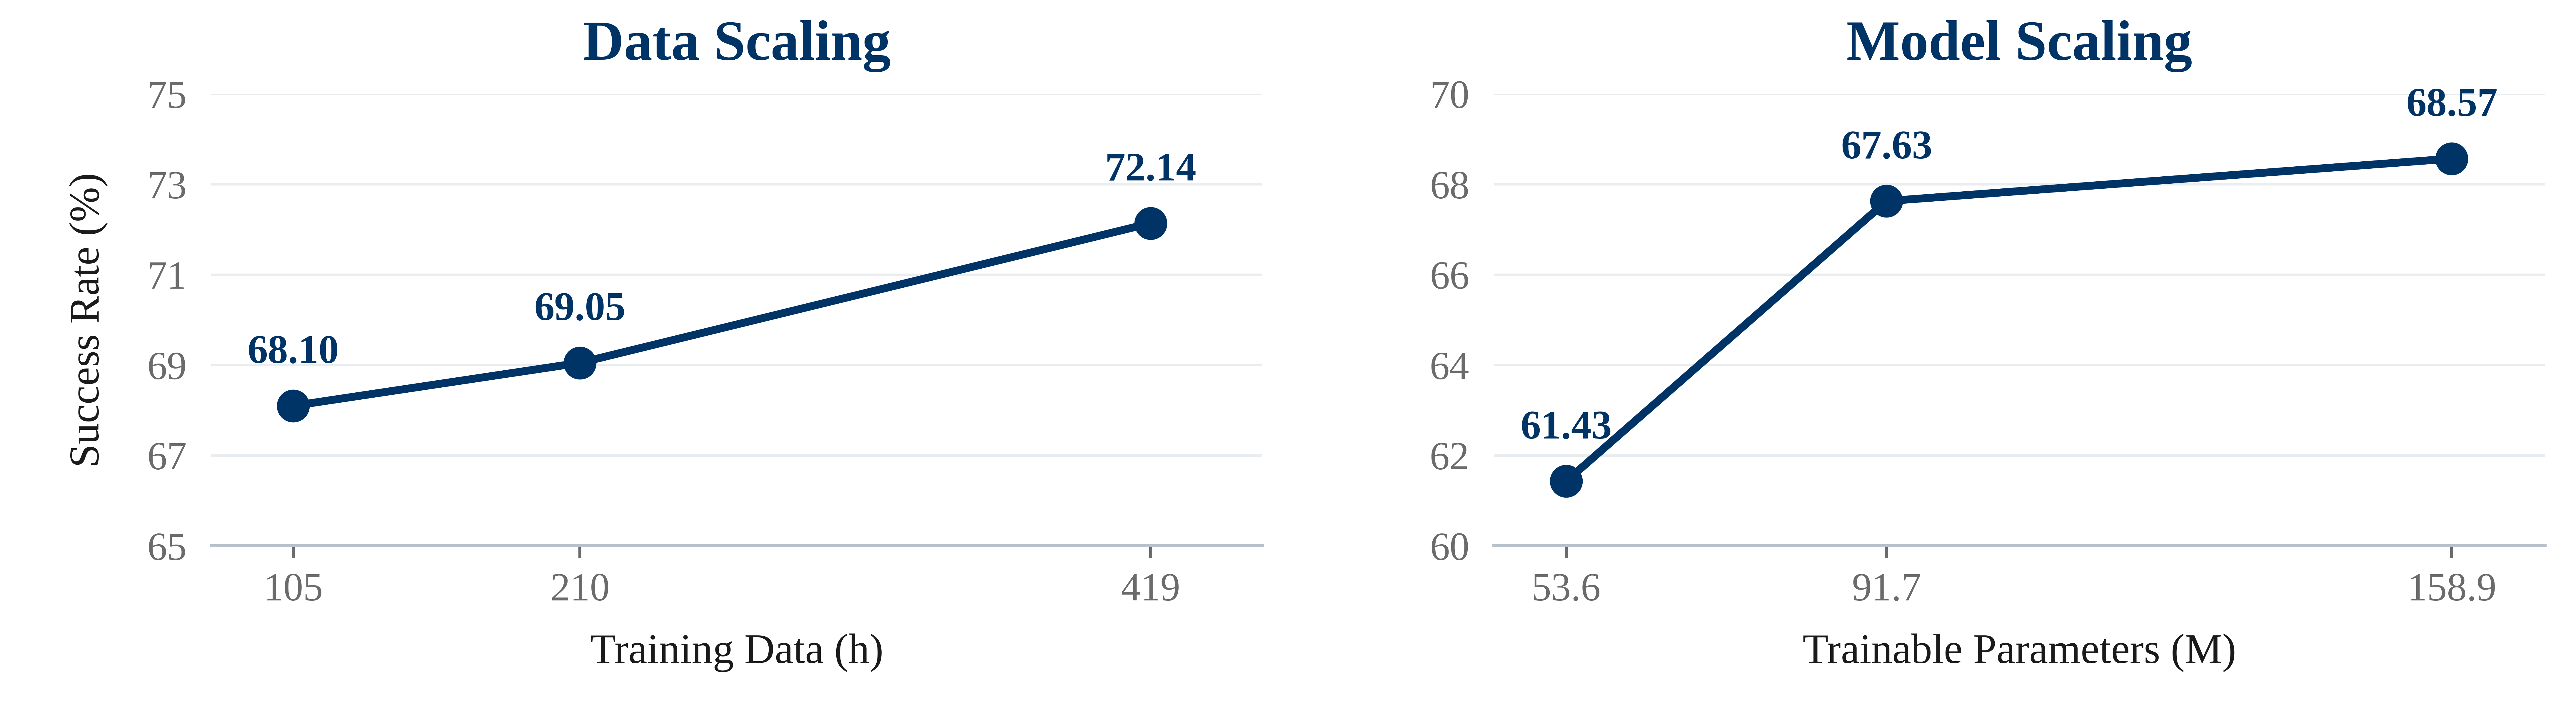
\includegraphics[width=\textwidth]{image/scaling_analysis.png}
  \caption{Scaling behavior of Kimodo-Policy. Left: overall success rate as a function of VLA policy-pretraining data duration. Right: overall success rate as a function of active policy parameters.}
  \label{fig:scaling_analysis}
\end{figure}

\textbf{Data scaling results.} Figure~\ref{fig:scaling_analysis} shows a consistent improvement as VLA policy-pretraining data increases: the overall success rate rises from 68.10\% with 105\,h to 69.05\% with 210\,h and 72.14\% with 419\,h, for a total gain of 4.04 percentage points. With the architecture, adaptation procedure, and evaluation protocol fixed, this trend demonstrates that Kimodo-Policy can translate additional humanoid demonstrations into stronger downstream control. In the proposed T2M-based framework, the pretrained motion prior supplies a structured basis for whole-body behavior, while broader VLA supervision improves how effectively visual observations and language instructions ground coordinated root, body, and hand actions. The consistent gains across the evaluated data scales point to further potential as larger and more diverse humanoid datasets become available.

\textbf{Model scaling results.} With the training data and optimization protocol held fixed, increasing active policy capacity yields higher overall success at every evaluated scale. The success rate improves from 61.43\% with 53.6M active parameters to 67.63\% with 91.7M, and reaches 68.57\% with 158.9M, for a 7.14-percentage-point gain from the smallest to the largest model. This improvement shows that additional capacity helps Kimodo-Policy represent multimodal conditioning and coordinate root, body, and hand predictions around its structured motion prior. The positive trend across all three configurations demonstrates that the proposed visually grounded, root--body--hand framework can benefit from increased capacity and motivates scaling to larger policies in conjunction with expanded training data.

\begingroup
% Use the official ICLR subsection formatting.
\subsection{Ablation Study}
\label{sec:exp_ablation}
\color{black}
We analyze the contribution of the pretrained T2M backbone, backbone freezing, VLA pretraining, the motion loss, and root--body gradient decoupling. All ablation variants are trained on a mixture of HumanoidArena tasks in the SONIC X7 setup and evaluated on DoubleDesk, Football, and P\&Pbox. Figure~\ref{fig:training_loss_comparison} shows the training-loss trajectories and the mean success rate across these three tasks for the corresponding model variants.
\begin{figure}[H]
  \centering
  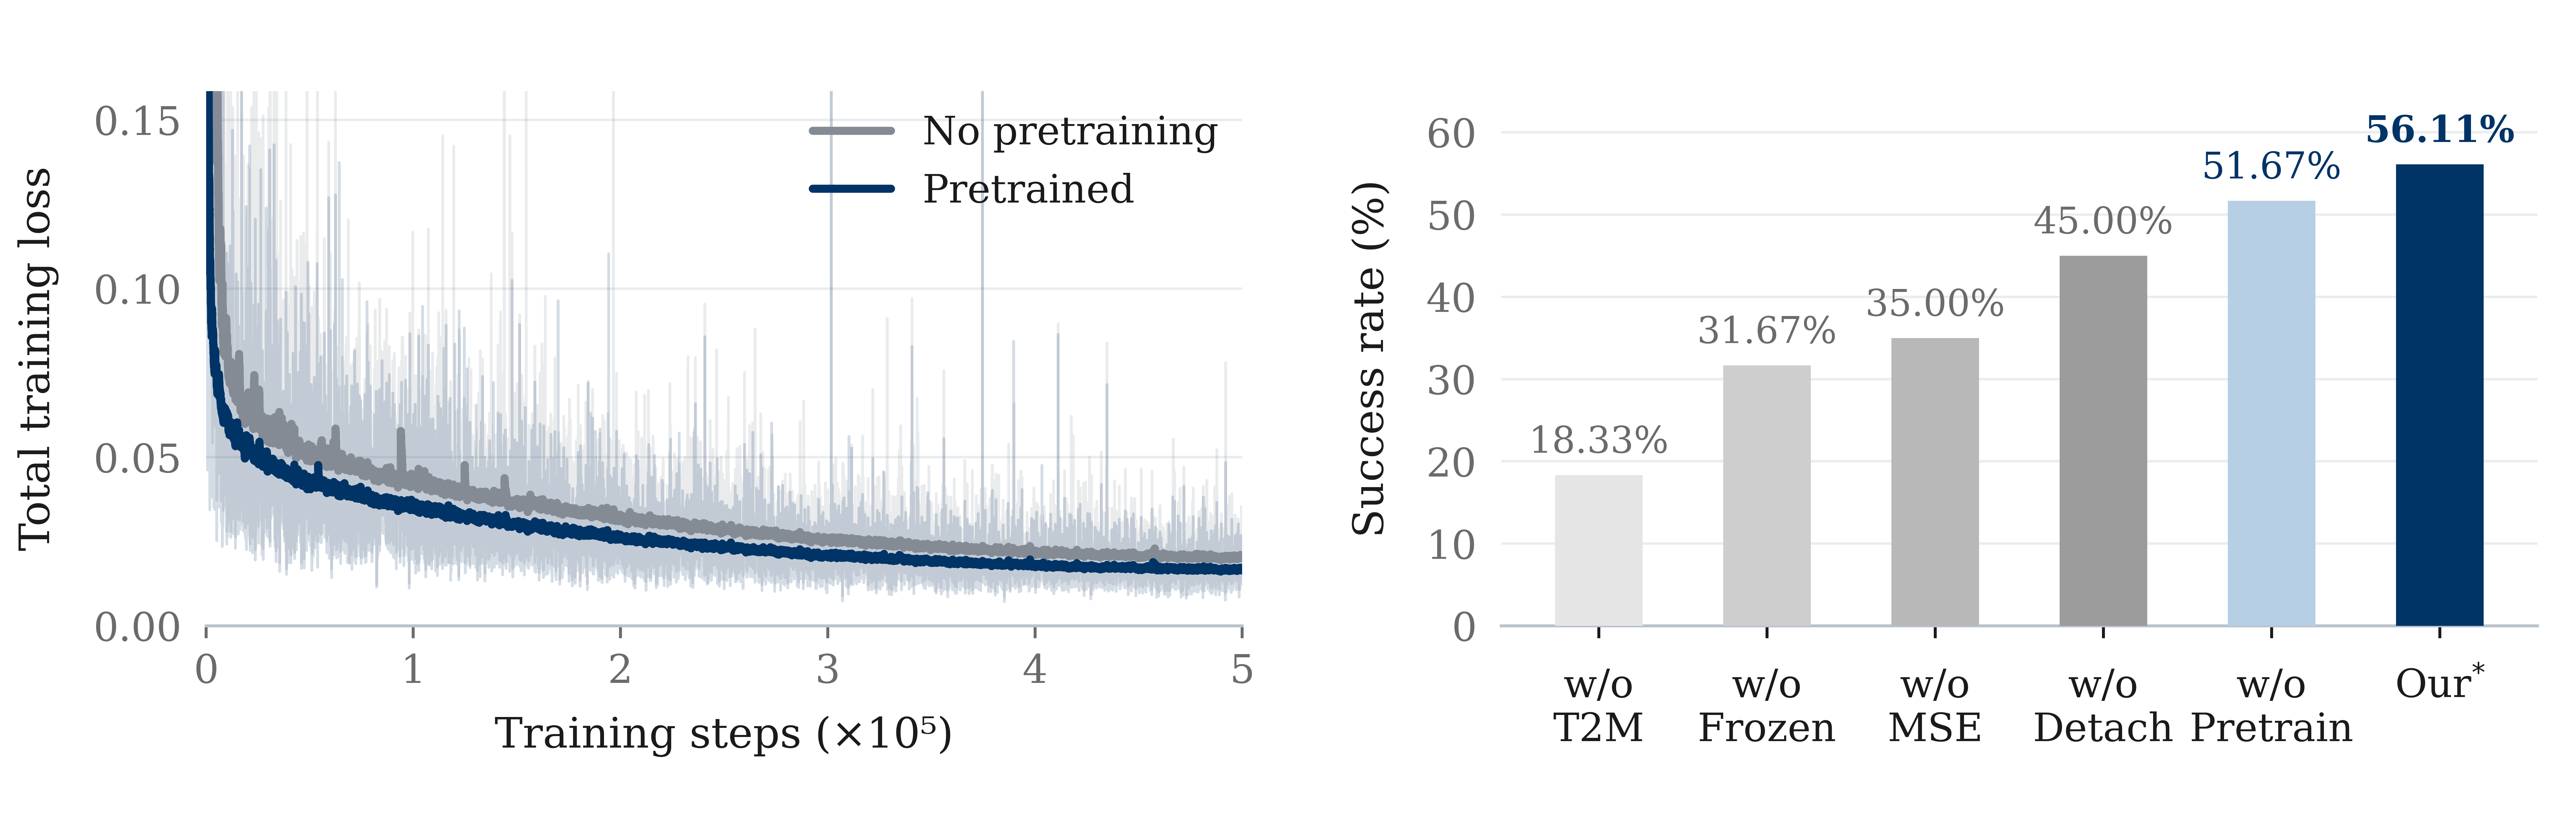
\includegraphics[width=\textwidth]{image/training_loss_comparison.png}
  \caption{\textbf{Training Dynamics and Ablation Performance.} Left: training-loss trajectories for the trained and no-training settings. Right: mean task success across DoubleDesk, Football, and P\&Pbox. Gray bars show component and training-design ablations: removing the T2M backbone (w/o T2M), unfreezing it (w/o Frozen), replacing MSE with the original Kimodo motion loss (w/o MSE), and removing root--body gradient detachment (w/o Detach). The VLA-pretraining comparison is shown separately in light blue (w/o Pretrain) and dark blue (Ours$^{*}$).}
  \label{fig:training_loss_comparison}
\end{figure}



\textbf{Effect of the pretrained motion prior and backbone freezing.} Without VLA pretraining, Kimodo-Policy achieves 51.67\% mean success. Removing the pretrained T2M backbone reduces success to 18.33\%, demonstrating the substantial contribution of the motion prior to downstream whole-body control. Unfreezing the backbone also degrades performance to 31.67\%, supporting the preservation of pretrained motion representations during policy adaptation. Together, these results validate our strategy of retaining a frozen motion generator while learning visual and task conditioning through dedicated trainable branches, enabling effective control without additional VLA pretraining.

\textbf{Effect of the prediction objective and root--body gradient decoupling.} Under the same setting without VLA pretraining, replacing MSE with the original Kimodo motion objective reduces success from 51.67\% to 35.00\%. This supports combining a preserved motion prior with direct supervision of policy prediction targets for downstream adaptation. Removing root--body gradient detachment further reduces success to 45.00\%. Detachment retains root-to-body conditioning while preventing the body loss from updating the root ControlNet, allowing each stage to learn through its own objective while preserving coordinated generation. These findings support direct prediction supervision and controlled cross-stage gradient flow as effective choices for adapting the structured motion prior to policy learning.

\textbf{Effect of VLA pretraining.} VLA pretraining further improves success from 51.67\% to 56.11\%, accompanied by generally lower training loss and smaller fluctuations. Since both variants retain the pretrained T2M backbone, this gain reflects the complementary benefit of learning visual and task conditioning beyond the motion prior itself. Collectively, the results support Kimodo-Policy's central design: preserving pretrained motion-generation capabilities, adapting them through dedicated conditioning branches and stage-specific optimization, and strengthening visually grounded control through VLA pretraining.


\endgroup
